\documentclass[10pt]{article}

\usepackage{amsthm}
\usepackage{amsmath}
\usepackage{amsfonts}
\usepackage{stmaryrd}
\usepackage{tikz}
\usepackage{comment}
\usetikzlibrary{shapes, arrows.meta, positioning}

\tikzstyle{block} = [draw, fill=white, rectangle]
\newtheorem{theorem}{Theorem}[section]
\newtheorem{lemma}{Lemma}[section]
\newtheorem{definition}{Definition}[section]

\newcommand{\code}[1]{\texttt{#1}}
\newcommand{\Z}{\mathbb{Z}}  % integers
\newcommand{\N}{\mathbb{N}}  % naturals
\newcommand{\B}{\mathbb{B}}  % booleans
% stream with elements of a given type
\newcommand{\stream}[1]{\ensuremath{\mathcal{S}_{#1}}}
% finite stream with elements of a given type (zero almost everywhere)
\newcommand{\streamf}[1]{\ensuremath{\overline{\mathcal{S}_{#1}}}}
\newcommand{\zm}{\ensuremath{z^{-1}}} % stream delay operator
\newcommand{\I}{\mathcal{I}}  % stream integration
\newcommand{\D}{\mathcal{D}}  % stream derivative
\newcommand{\distinct}{\mathit{distinct}}  % distinct operator
\newcommand{\q}{\ensuremath{\mathcal{Q}}}  % query
% multiset of elements with given type
\newcommand{\multiset}[1]{\mathit{multiset}_{#1}}
% set with elements of given type
\newcommand{\set}[1]{\mathit{set}_{#1}}
\newcommand{\id}{\ensuremath{\mathit{id}}} % identity function
\newcommand{\isset}{\mbox{isset}}
\newcommand{\ispositive}{\mbox{ispositive}}

\title{Streaming Differential Datalog}

\begin{document}
\maketitle

\section{Basic notation}

\begin{comment}
\subsection{Types}

$\N$ is the set of natural numbers, while $\Z$ is the set of integers.

Our language will deal with a set of base types $B$ that includes
$\N$, $\Z$, \code{string}, $\B$ (Booleans), $\mathbf{unit}$.

Derived types include: tuples, vectors (lists), functions.

$$T = B \;|\; T \times T \;|\; T^* \;|\; T \rightarrow T$$

%% We also highlight two special derived types: $\multiset{T}$: finite
%% multisets of elements of type $T$, and $\set{T}$: sets of elements of
%% type $T$.  We call these two particular types \emph{collections}.

A typing context is a map that assigns types to variable names.
$\Gamma = x_1 : T_1, x_2 : T_2, \ldots, x_m : T_m$, where $T_i$ is the
type of variable $x_i$.
\end{comment}

\subsection{Monoids and groups}

A monoid $(M, 0_M, +_M)$ is a set $M$ with a distinguished element
$0_M \in M$ and a binary associative operation $+_M : M \times M
\rightarrow M$, such that $a +_M 0 = 0 +_M a = a$ for any $a \in M$.
When clear from the context we drop the index $_M$.  A commutative
monoid has the property that $a + b = b + a$ for all $a, b \in M$.  A
group is a monoid where every element $a \in M$ has a complement $-a
\in M$ such that $a + (-a) = 0$.

\subsection{Multisets}

Given a monoid (group) $B$, the set of functions between $A$ and $B$
form a monoid (group): M = $A \rightarrow B$, defined by $0_M = (x
\mapsto 0_B)$ and $f +_M g = x \mapsto f(x) +_B g(x)$.  If $B$ is a
monoid (group), we denote the \emph{finite} functions between $A$ and
$B$ as $B[A]$; these are functions where $f(x) \not= 0_B$ for at most
a finite number of values of $x \in A$.  Such a function can be
denoted by enumerating the inputs that map to non-zero values: $\{ x_1
\mapsto b_1, \dots, x_n \mapsto b_n \}$.  The values in $B[A]$ can
also be thought as being key-value maps with keys in $A$ and values in
$B$.

In particular, \emph{multisets} with elements of type $A$ are the
functions $\Z[A]$.  Multiset union is just addition in the $\Z[A]$
monoid.  Note that multisets elements can have negative weights.
Multisets form a commutative group, since $\Z$ with addition is a
group.  The zero is the empty multiset $\{\} = \phi$.  Given a
multiset $m \in \Z[A]$ and a value $v \in A$, we overload the array
index notation $m[v]$ to denote the \emph{weight} of the element $v$
in $m$.

The ``distinct'' function $\distinct: \Z[D] \rightarrow \Z[D]$
projects a multiset into an underlying set (but \emph{the result is
  still as a multiset}).  The definition of distinct is given by
$\distinct(m) = \{ x \mapsto 1, m[x] > 0 \} \in \Z[D]$.  The distinct
function is idempotent: $\distinct = \distinct \circ \distinct$.

We say that a multiset is also a ``set'' if the weight of every
element is either zero or one: $\isset : \Z[D] \rightarrow \B$,
given by

$$\isset(s) = \left\{
\begin{array}{ll}
  \mbox{true} & \mbox{ if } s[x] \in \{ 0, 1 \}, \forall x \in D \\
  \mbox{false} & \mbox{ otherwise}
\end{array}
\right.$$

Node that $\isset(s) \iff s = \distinct(s)$.

We say that a multiset is positive if the weight of every element is
positive: $\ispositive : \Z[D] \rightarrow \B$, given by

$$\ispositive(s) = \left\{
\begin{array}{ll}
  \mbox{true} & \mbox{ if } s[x] \geq 0, \forall x \in D \\
  \mbox{false} & \mbox{ otherwise}
\end{array}
\right.$$

Note that for any $m \in \Z[D]$ we have: $\isset(\distinct(m))$
and $\ispositive(\distinct(m))$.  We also write $m \geq 0$ when
$m$ is positive.  We also say that $m \geq n$ for $m, n \in \Z[D]$ if
$m - n \geq 0$.

We call a function (query) between multisets ``linear'' if it commutes
with addition: $\q: \Z[I] \rightarrow \Z[O]$ has the property that
$\q(a +_{\Z[I]} b) = \q(a) +_{\Z[O]} \q(b)$ for any $a, b \in \Z[I]$.
This implies that for a linear query $\q(0_{\Z[I]}) = 0_{\Z[O]}$.

\subsection{Streams}

Given a monoid $T$, streams $\stream{T}$ of values of type $T$ are
functions $\N \rightarrow T$.  We often think of the index in $\N$ as
being time; if $s \in \stream{T}$ is a stream of values of type $T$,
the notation $s[t] = s(t) \in T$ denotes the value of the element of
the stream $s$ ``at time'' $t \in \N$.  To simplify some proofs we
define that $s[-1] = 0_T$.

Functions on monoids can be ``lifted'' to operate on streams: given
$f: I \rightarrow O$ we can extend it on streams pointwise: $f :
\stream{I} \rightarrow \stream{I}$ given by $o[t] = f(i)[t] = f(i[t])$.

We depict the streams as arrows, and the pointwise application of a
function to stream as a box, as in the following diagram:

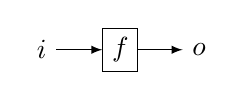
\begin{tikzpicture}[auto,node distance=1cm,>=latex]
    \node [] (input) {$i$};
    \node [block, right of=input] (f) {$f$};
    \node [right of=f] (output) {$o$};
    \draw [->] (input) -- (f);
    \draw [->] (f) -- (output);
\end{tikzpicture}

This works also for functions with multiple inputs, e.g.  a function
$f: A \times B \rightarrow C$ can be lifted to operate on streams $f:
\stream{A} \times \stream{B} \rightarrow \stream{C}$ computing
pointwise on time: $f(a, b)[t] = f(a[t], b[t])$ for $t \in \N$.

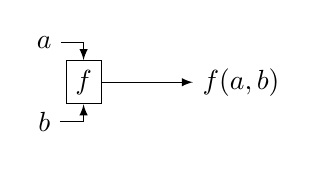
\begin{tikzpicture}[auto,node distance=.5cm,>=latex]
  \node [] (input1) {$a$};
  \node [below of=input1] (midway) {};
  \node [below of=midway] (input2) {$b$};
  \node [block, right of=midway] (f) {$f$};
  \node [right of=f, node distance=2cm] (output) {$f(a,b)$};
  \draw [->] (input1) -| (f);
  \draw [->] (input2) -| (f);
  \draw [->] (f) -- (output);
\end{tikzpicture}

The $\zm: \stream{T} \rightarrow \stream{T}$ \emph{delay operator} is
a function from streams to streams, defined as
$$(\zm(s))[t] = \left\{
\begin{array}{ll}
  0_T & \mbox{ if } t = 0 \\
  s[t - 1] & \mbox{ for } t > 0.
\end{array}
\right.
$$

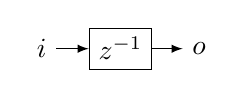
\begin{tikzpicture}[auto,node distance=1cm,>=latex]
    \node [] (input) {$i$};
    \node [block, right of=input] (z) {$\zm$};
    \node [right of=z] (output) {$o$};
    \draw [->] (input) -- (z);
    \draw [->] (z) -- (output);
\end{tikzpicture}

We write $z^{-k}$ for $\underbrace{\zm \circ \ldots \circ \zm}_{k
  \mbox{ times}}$ .

We call a function over streams \textbf{memoryless} if it has the
property: $f \circ \zm = \zm \circ f$.

\begin{definition}
Given a monoid $M$, \textbf{integration} is an operation from streams to
streams, $\I : \stream{M} \rightarrow \stream{M}$.  The integral of a
stream $S$ is defined using an equation: $\I(s) = \zm(\I(s)) + s$.
(Using the notation used for digital filters this equation can be also
written as $\I(s) = s / (1 - \zm)$).  The element of $\I(s)$ at time
$t$ is the (prefix) sum of all elements of $s$ at times up to $t$:
$\I(s)[t] = \sum_{i \leq t} s[t]$, where the sum uses the addition of
the underlying monoid $M$.  The digital filter for $\I$ is given in
the following figure:

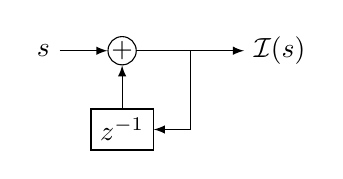
\begin{tikzpicture}[auto,>=latex]
    \node [] (input) {$s$};
    \node [block, shape=circle, right of=input, inner sep=0pt] (plus) {$+$};
    \node [right of=plus, node distance=2cm] (output) {$\I(s)$};
    \node [block, below of=plus, node distance=1cm] (z) {$z^{-1}$};
    \draw [draw,->] (input) -- (plus);
    \draw [->] (plus) -- node (o) {} (output);
    \draw [->] (o) |- (z);
    \draw [->] (z) -- (plus);
\end{tikzpicture}
\end{definition}

\begin{definition}
Given a group $M$, \textbf{differentiation} is an operation from
streams to streams $\D : \stream{M} \rightarrow \stream{M}$, defined
as $\D(s) = s - \zm(s)$ (we need $M$ to be group in order to have
subtraction).  An element of $\D(s)$ (at time $t$) is the difference
between the previous element (time $t-1$) of $s$ and the current (time
$t$) element of $S$.  Using the notation for digital filters $\D(s) =
s(1 - \zm)$.

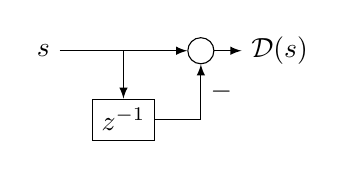
\begin{tikzpicture}[auto,>=latex]
    \node [] (input) {$s$};
    \node [block, shape=circle, right of=input,node distance=2cm] (plus) {};
    \node [right of=plus] (output) {$\D(s)$};
    \draw [draw,->] (input) -- node (i) {} (plus);
    \node [block, below of=i, node distance=1cm] (z) {$\zm$};
    \draw [->] (plus) -- (output);
    \draw [->] (i) -- (z);
    \draw [->] (z) -| node[near end,right] {$-$} (plus);
\end{tikzpicture}
\end{definition}

\begin{lemma}
For a stream $s$ over a commutative group we have $D(I(s)) = s$.
\end{lemma}
\begin{proof}
$\D(\I(s)) = \I(s) - \zm(\I(s)) = (\zm(\I(s)) + s) - \zm(\I(s)) = s$, by
  substituting the definitions of $\D$ and $\I$ and using the
  commutativity of the group.
\end{proof}

If $I$ and $O$ are monoids, we call an operator $f: \stream{I}
\rightarrow \stream{O}$ over streams \textbf{linear} if $\forall t \in
\N . f(a +_I b)[t] = (f(a) +_O f(b))[t]$.  Notice that this is a
different kind of linearity than the linearity of operators between
multisets: this is linearity in the time dimension.  The following
observation is trivial: the stream operator produced by lifting a
linear function between monoids $f: I \rightarrow O$ is also linear.
The operator $\zm$ is linear.

\begin{lemma}
  The composition of two linear stream operators is linear.
\end{lemma}
\begin{proof}
  For suitable monoids $I, O, P$, consider two linear operators $f:
  \stream{I} \rightarrow \stream{O}$ and $g: \stream{O} \rightarrow
  \stream{P}$.
$$
\begin{aligned}
  g(f(a +_I b))[t] &= g(f(a) +_O f(b))[t] & \mbox{ linearity of }f \\
  &= (g(f(a)) +_P g(f(b)))[t] & \mbox{ linearity of }g. \\
\end{aligned}
$$
\end{proof}

\begin{lemma}
  The composition of two memoryless stream operators is memoryless.
\end{lemma}
\begin{proof}
  For suitable sets $I, O, P$, consider two memoryless operators $f:
  \stream{I} \rightarrow \stream{O}$ and $g: \stream{O} \rightarrow
  \stream{P}$.
$$
\begin{aligned}
  \zm(g(f(i))) &= g(\zm(f(i))) & \mbox{ since $g$ is memoryless} \\
  &= g(f(\zm(i))) & \mbox{ since $f$ is memoryless}.
\end{aligned}
$$
\end{proof}

\begin{lemma}
  When computing over a commutative group, the operators $\I$, $\D$,
  and $\zm$ are memoryless and linear.
\end{lemma}
\begin{proof}
  $\D$ is the composition of three linear and memoryless operators.
  For $\zm$ the proof is trivial.
  $$
\begin{aligned}
  \zm(\I(i))[t] &= \zm(\sum_{k \leq t} i[k]) & \mbox{ definition of }\I \\
  &= \sum_{k \leq t-1} i[k] & \mbox{ definition of }\zm \\
  &= \sum_{k \leq t} \zm(i[k]) & \mbox{ commutativity }\zm \\
  &= \I(\zm(i))[t] & \mbox{ definition of }\I. \\
  (\I(a + b))[t] &= \sum_{k \leq t}(a + b)[t] & \mbox{ definition of }\D \\
  &= \sum_{k \leq t} a[k] + \sum_{k \leq t} b[k] & \mbox{ commutativity, linearity of + } \\
  &= \I(a)[t] + \I(b)[t] & \mbox{ definition of }\I.
\end{aligned}
$$
\end{proof}

\subsection{Loops as streams}

We introduce two new operators that can create streams and convert a
stream to a scalar value.

The Kroneker delta function $\delta_0 : T \rightarrow \stream{T}$
produces a stream from a scalar value.  The stream is
defined:

$$\delta_0(v)[t] = \left\{
\begin{array}{ll}
  v & \mbox{if } t = 0 \\
  0_T & \mbox{ otherwise}
\end{array}
\right.
$$

We diagram the $\delta_0$ operator using a dotted arrow as input, since
the input is a scalar value.

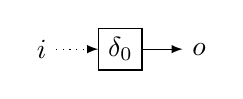
\begin{tikzpicture}[auto,node distance=1cm,>=latex]
    \node [] (input) {$i$};
    \node [block, right of=input] (delta) {$\delta_0$};
    \node [right of=delta] (output) {$o$};
    \draw [->,dotted] (input) -- (delta);
    \draw [->] (delta) -- (output);
\end{tikzpicture}

Let us denote with $\streamf{T}$ streams that are almost everywhere
(a.e.)  $0_T$ (only a finite number of values in the stream have a
non-zero value).  We define a function $\int : \streamf{T} \rightarrow
T$ as $\int(s) = \sum_{t \geq 0} s[t]$.

We can also extend the set $T$ with an ``infinite'' value $\top$:
$\overline{T} = T \cup \{ \top \}$, and define $\int{s} = \top$ for
streams $s \in \stream{T} \setminus \streamf{T}$.

\begin{tikzpicture}[auto,node distance=1cm,>=latex]
    \node [] (input) {$i$};
    \node [block, right of=input] (S) {$\int$};
    \node [right of=delta] (output) {$o$};
    \draw [->] (input) -- node {$do$} (S);
    \draw [->, dotted] (S) -- (output);
\end{tikzpicture}

\subsection{Streams over multisets}

In the rest of this text we consider only streams over multisets
$\stream{\Z[T]}$, for some type of element $T$: at each time moment the
value of the stream is a multiset.  Since multisets form a commutative
group, addition and subtraction on streams over multisets of the same
type are well-defined.

\begin{definition}
A stream over a multiset is \textbf{monotone} if $s[t] \geq s[t-1],
\forall t \in \N$.
\end{definition}

\begin{lemma}
Given a positive stream $s$ over a group, the stream $\I(s)$ is
monotone.
\end{lemma}
\begin{proof}
  Let us compute $\I(s)[t + 1] - \I(s)[t] = \sum_{i \leq t+1}s[i] -
  \sum_{i \leq t}s[i] = s[t+1] \geq 0$, by commutativity.
\end{proof}

\begin{lemma}
Given a monotone stream $s$ over a group, the elements of the stream
$\D(s)$ are positive.
\end{lemma}
\begin{proof}
  By the definition of monotonicity $s[t+1] \geq s[t]$.  By definition
  of $\D$ we have $\D(s)[t+1] = s[t+1] - s[t] \geq 0$.
\end{proof}

\section{A semantics of Datalog in terms of streams}

Let us consider a language that consists of the relational algebra
together with stratified negation and recursive definitions.  Let us
consider a query $\q$ in this language.  Let us assume that the query
defines a function $\q : I \rightarrow O$, where $I$ and $O$ are
multisets with elements from a fixed universe.  We can naturally
``lift'' the semantics of $q$ to compute on $\stream{I} \rightarrow
\stream{O}$ pointwise: $q(i)[t] = q(i[t]), \forall t \geq 0, \mbox {
  for } i \in \stream{I}$.  Note that the semantics of Datalog
promises that once an input is a set, the output is also a set.

\begin{theorem}
Consider a recursive datalog query of the form: $o = i \cup \q(o)$,
where $\q$ is a relational query.  The following filter implements the
Datalog set semantics of $o$:

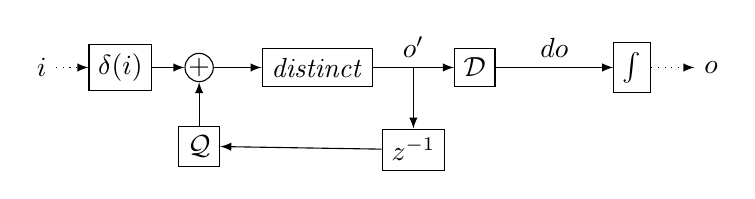
\begin{tikzpicture}[auto,>=latex]
  \node [] (input) {$i$};
  \node [block, right of=input] (delta) {$\delta(i)$};
  \node [block, shape=circle, right of=input, node distance=2cm, inner sep=0in] (plus) {$+$};
  \node [block, right of=plus, node distance=1.5cm] (distinct) {$\distinct$};
  \node [block, right of=distinct,node distance=2cm] (D) {$\D$};
  \node [block, right of=D, node distance=2cm] (S) {$\int$};
  \node [right of=S] (output)  {$o$};
  \node [block, below of=plus, node distance=1cm] (f) {$\q$};
  \draw [->, dotted] (input) -- (delta);
  \draw [->] (delta) -- (plus);
  \draw [->] (plus) -- (distinct);
  \draw [->] (distinct) -- node (o) {$o'$} (D);
  \draw [->] (D) -- node (do) {$do$} (S);
  \draw [->, dotted] (S) -- (output);
  \node [block, below of=o, node distance=1.3cm] (z) {$\zm$};
  \draw [->] (o) -- (z);
  \draw [->] (z) -- (f);
  \draw [->] (f) -- (plus);
\end{tikzpicture}
\end{theorem}
\begin{proof}
  TODO
\end{proof}

Since $\q$ is a relational query, we have that $i \geq 0 \Rightarrow
\q(i) \geq 0$.  We can prove using induction over time that the stream
$o'$ (the output of the $\distinct$ block) is monotone.  Thus the
stream defined by the output of $\D$ block is positive.  If there is a
$t$ such that $o'[t + 1] = o'[t]$, if follows that $o'[t + k] = o'[t]$
for all $k \geq 0$, which implies that the stream $do$ is 0 a.e., and
thus $o$ is well-defined.  Moreover, we can prove that $\isset(o)$.

Let us notice that the combination $\int \circ \D$ applied to a
monotone stream will produce that fixed-point value of the input
stream (if it exists).  Under this circumstance the output of the
$\int$ corresponds to its first $0$ input.

\section{Differential Datalog}

\begin{definition}
Consider a traditional datalog program $\q: I \rightarrow O$, where
$I$ and $O$ are multiset types.  When this program is considered as a
Differential Datalog program it's semantics is a function $\q:
\stream{I} \rightarrow \stream{O}$, defined by the following diagram:
$\D \circ \q \circ \I$.
\end{definition}  Notice that, while the original program computes on
multisets, the DDlog program computes on streams of multisets.

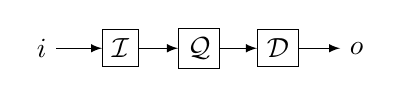
\begin{tikzpicture}[auto,node distance=1cm,>=latex]
    \node [] (input) {$i$};
    \node [block, right of=input] (I) {$\I$};
    \node [block, right of=I] (q) {$\q$};
    \node [block, right of=q] (D) {$\D$};
    \node [right of=D] (output) {$o$};
    \draw [->] (input) -- (I);
    \draw [->] (I) -- (q);
    \draw [->] (q) -- (D);
    \draw [->] (D) -- (output);
\end{tikzpicture}

Note that the definition uses the ``lifted'' implementation of the
program $\q$, operating over streams.

Also note that if program $\q$ contains a fixed-point sub-query, then
the implementation of $\q$ contains a block that computes over a
stream of streams!  We will denote a stream where each element is a
stream with a double arrow.  Then the previous query $o = i \cup
\q(o)$ provides the following DDlog program:

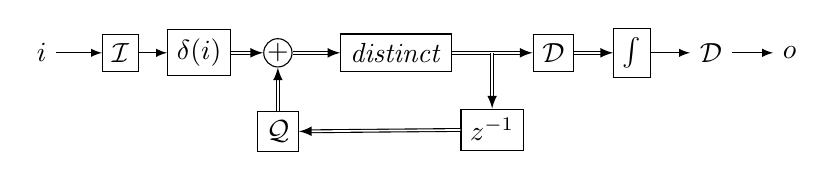
\begin{tikzpicture}[auto,>=latex]
  \node [] (input) {$i$};
  \node [block, right of=input] (I) {$\I$};
  \node [block, right of=I] (delta) {$\delta(i)$};
  \node [block, shape=circle, right of=I, node distance=2cm, inner sep=0in] (plus) {$+$};
  \node [block, right of=plus, node distance=1.5cm] (distinct) {$\distinct$};
  \node [block, right of=distinct,node distance=2cm] (D) {$\D$};
  \node [block, right of=D] (S) {$\int$};
  \node [right of=S] (D2) {$\D$};
  \node [right of=D2] (output)  {$o$};
  \node [block, below of=plus, node distance=1cm] (f) {$\q$};
  \draw [->] (input) -- (I);
  \draw [->] (I) -- (delta);
  \draw [->, double] (delta) -- (plus);
  \draw [->, double] (plus) -- (distinct);
  \draw [->, double] (distinct) -- node (o) {} (D);
  \draw [->, double] (D) -- (S);
  \draw [->] (S) -- (D2);
  \draw [->] (D2) -- (output);
  \node [block, below of=o, node distance=1.1cm] (z) {$\zm$};
  \draw [->, double] (o) -- (z);
  \draw [->, double] (z) -- (f);
  \draw [->, double] (f) -- (plus);
\end{tikzpicture}

\section{Term-rewriting transformations}

To implement efficiently a DDlog program the compiler makes use of a
series of term-rewriting transformations.  We list here some of them.

\subsection{Linear queries}

\begin{theorem}
If $\q$ is a linear query, we have: $\q \circ \I = \I \circ \q$ and
$\D \circ \q = \q \circ \D$.
\end{theorem}
\begin{proof}
$$
\begin{aligned}
  ((\q \circ \I)(i))[t] &= \q(\sum_{i \leq t} i[t]) & \mbox{by definition of }\I \\
  &= \sum_{k \leq t} \q(i[k]) & \mbox{by linearity of }\q \\
  &= \I(\q(i))[t] & \mbox{by definition of }\I. \\
  ((\D \circ \q)(i))[t] &= \q(i[t]) - \q(i[t-1]) & \mbox{by definition of }\D \\
  &= \q(i[t] - i[t-1]) & \mbox{by linearity of }\q \\
  &= \q(\D(i)))[t] & \mbox{by definition of }\D.
\end{aligned}
$$
\end{proof}

Using this observation it follows that for linear programs $\q$ the
DDlog implementation is the same as the Datalog implementation:

$\D(\q(\I(i))) = \q(\D(\I(i))) = \q(i)$.

\subsection{Bi-linear queries}

Consider a bi-linear query of two inputs: $\q : \Z[I] \times
\Z[J] \rightarrow \Z[O]$ with the properties: $\q(a + b, c) = \q(a,
c) + \q(b, c)$ and $\q(a, c + d) = \q(a, c) + \q(a, d)$.  Cartesian
products and joins have this property.  For such a query we have the
following property:

\begin{theorem}
  If $\q$ is a bi-linear query, we have:
  $$
  \begin{aligned}
    \q(\I(a), \I(b)) &= \zm(\q(\I(a)), \I(b)) + & \mbox{ ``previous''
      version of }\q \\
    &= \q(\I(\zm(a)), b) +& \mbox{ uses previous version of left input}\\
    &= \q(a, \I(\zm(b))) + & \mbox{ uses previous version of right input} \\
    &= \q(a, b) & \mbox{ only based on latest changes}.
  \end{aligned}
$$
\end{theorem}
\begin{proof}
  The proof is based on algebraic manipulations starting from the
  definition of $\I(a) = \zm(\I(a)) + a$ using the memoryless properties.
\end{proof}

\subsection{Recursion}

TODO

\hrule
\hrule
\pagebreak

From now on this is WIP.

\begin{comment}
\subsection{DDlog types}

\[\frac{\code{A}: T, \code{B}: S}{\code{(A,B)}: T \times S}\]
\[\frac{\code{A}: T, \code{B}: S}{\code{function(x:A):B}: A \rightarrow B}\]
\[\frac{\code{T1}: T_1, \code{T2}: T_2}{\code{T1 | T2} : T_1 \oplus T_2}\]
\[\frac{\code{T1}: T_1, \code{T2}: T_2}{\code{Constructor\{f1: T1, f2:
    T2\}} : \string \rightarrow T_1 \oplus T_2}\]
\end{comment}

\subsection{DDlog collections}

DDlog programs consume and produce streams of data.  The outside world
inputs/outputs streams feed to/from DDlog collections.  A DDlog
transaction defines a time step for all the input streams.  On each
transaction commit DDlog updates all output streams.  DDlog programs
only operate on streams.  Some input and output streams are fed
directly to DDlog programs, while others are processed, as described
in this section.

\subsubsection{\code{input stream IS[D]}}

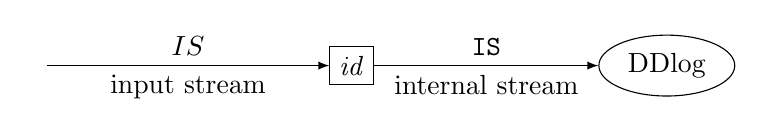
\begin{tikzpicture}[auto, node distance=4cm,>=latex]
    \node [] (input) {};
    \node [block, right of=input] (block) {\id};
    \node [block, shape=ellipse, right of=block] (ddlog) {DDlog};
    \draw [draw,->] (input) -- node {$IS$} (block) node [below,pos=0.5] {input stream};
    \draw [->] (block) -- node {$\code{IS}$}(ddlog) node [below,pos=0.5] {internal stream};
\end{tikzpicture}

A DDlog declaration of \code{input stream IS[D]} declares a (DDlog
internal) stream $\code{IS} \in \stream{\Z[\code{D}]}$, where the
stream's elements are multisets with elements of type \code{D}.  Given
a stream of input values $IS \in \stream{\Z[D]}$, the contents of the
DDlog stream \code{IS} is exactly $IS$.  $\id$ is the identity
function on streams $\id(x) = x$.

\subsubsection{\code{output stream OS[D]}}

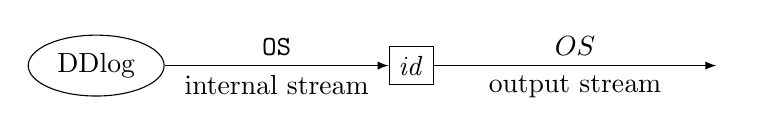
\begin{tikzpicture}[auto, node distance=4cm,>=latex]
    \node [block, shape=ellipse] (ddlog) {DDlog};
    \node [block, right of=ddlog] (block) {\id};
    \node [right of=block] (output) {};
    \draw [draw,->] (ddlog) -- node {\code{OS}} (block) node [below,pos=0.5] {internal stream};
    \draw [->] (block) -- node {$OS$}(output) node [below,pos=0.5] {output stream};
\end{tikzpicture}

As shown in the previous diagram, a DDlog declaration of \code{output
  stream OS[D]} declares an (output) stream $OS \in
\stream{\Z[\code{D}]}$.  The contents of the output stream $OS$ is
exactly the contents of the stream \code{OS}.

\subsubsection{\code{input multiset IM[D]}}

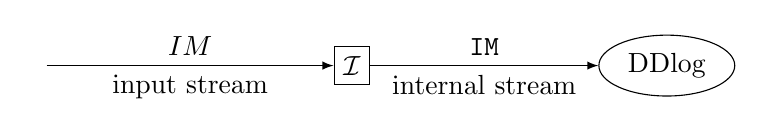
\begin{tikzpicture}[auto, node distance=4cm,>=latex]
    \node [] (input) {};
    \node [block, right of=input] (block) {$\I$};
    \node [block, shape=ellipse, right of=block] (ddlog) {DDlog};
    \draw [draw,->] (input) -- node {$IM$} (block) node [below,pos=0.5] {input stream};
    \draw [->] (block) -- node {$\code{IM}$}(ddlog) node [below,pos=0.5] {internal stream};
\end{tikzpicture}

A DDlog declaration of \code{input multiset IM[D]} declares a stream
$\code{IM} \in \stream{\Z[\code{D}]}$.  Given a stream of input values
$IM \in \stream{\Z[\code{D}]}$, the contents of \code{IM} is given by
$\code{IM} = \I(MI)$, the integral of the stream of inputs.

\subsubsection{\code{output multiset OM[D]}}

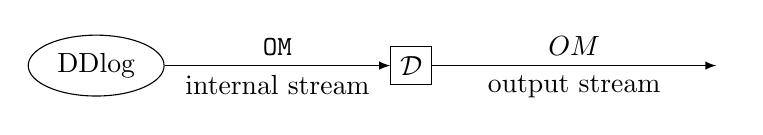
\begin{tikzpicture}[auto, node distance=4cm,>=latex]
    \node [block, shape=ellipse] (ddlog) {DDlog};
    \node [block, right of=ddlog] (block) {$\D$};
    \node [right of=block] (output) {};
    \draw [draw,->] (ddlog) -- node {\code{OM}} (block) node [below,pos=0.5] {internal stream};
    \draw [->] (block) -- node {$OM$}(output) node [below,pos=0.5] {output stream};
\end{tikzpicture}

A DDlog declaration of \code{output multiset OM[D]} declares a stream
$OM \in \stream{\Z[\code{D}]}$.  The contents of the (output) stream
$OM$ is given by $OM = \D(\code{OM})$, the derivative of the stream
\code{OM}.

\subsubsection{\code{input relation IR[D]}}

\begin{tikzpicture}[auto, node distance=4cm,>=latex]
    \node [] (input) {};
    \node [block, right of=input] (distinct) {$\distinct$};
    \node [block, right of=distinct] (I) {$\I$};
    \node [block, shape=ellipse, right of=I] (ddlog) {DDlog};
    \draw [draw,->] (input) -- node {$IR$} (block) node [below,pos=0.5] {input stream};
    \draw [draw,->] (distinct) -- (I);
    \draw [->] (I) -- node {$\code{IR}$}(ddlog) node [below,pos=0.5] {internal stream};
\end{tikzpicture}

A DDlog declaration of \code{input relation IR[D]} declares a stream
$\code{IR} \in \stream{\Z[\code{D}]}$.  The elements of the stream
\code{IR} are defined by $\code{IR} = \distinct(\I(IR))$.

\subsubsection{\code{output relation OR[D]}}

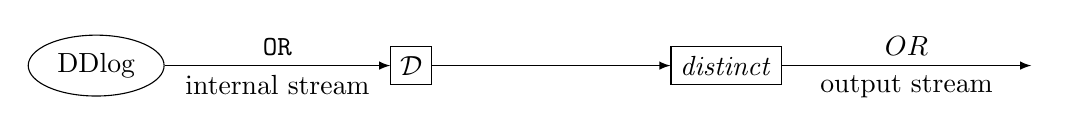
\begin{tikzpicture}[auto, node distance=4cm,>=latex]
    \node [block, shape=ellipse] (ddlog) {DDlog};
    \node [block, right of=ddlog] (D) {$\D$};
    \node [block, right of=D] (distinct) {$\distinct$};
    \node [right of=distinct] (output) {};
    \draw [draw,->] (ddlog) -- node {\code{OR}} (D) node [below,pos=0.5] {internal stream};
    \draw [draw,->] (D) -- (distinct);
    \draw [->] (distinct) -- node {$OR$}(output) node [below,pos=0.5] {output stream};
\end{tikzpicture}

A DDlog declaration of \code{output relation OR[D]} declares a stream
$OR \in \stream{\Z[\code{D}]}$.  The elements of the stream are $OR$ are defined
by $OR = \D(\distinct(\code{OR}))$.

\subsection{DDlog operators}

All DDlog operators: join, group-by, aggregate, projection, etc., are
just particular instances of functions over multisets.  When computing
over streams DDlog just applies these functions to the streams
pointwise.  In this section we describe the semantics of these
operators over a multi-set; the semantics over streams is just lifted
pointwise.

\subsection{DDlog syntax}

A Datalog rule is a term of the form:

\begin{eqnarray*}
  rule &::=& atom \code{ :- } \mathit{RHSClauses}. \\
  atom &::=& C[X] \mbox{ where $C$ is a collection and $X$ is a tuple
    of names} \\
  \mathit{RHSClauses} &::=& \mathit{RHSClause} \\
  &|& \mathit{RHSClause}, \mathit{RHSClauses} \\
  \mathit{RHSClause} &::=& \code{not } atom \\
  &|& expr   \\
  &|& \code{var } name = expr \\
  &|& \code{var } name = \code{FlatMap}( expr ) \\
  &|& \code{var } name = expr \code{.groupby}( expr ) \\
\end{eqnarray*}

\end{document}
